\documentclass{article}
\usepackage[utf8]{inputenc}

% \title{CS7350HW2}
%\author{byleve2022 }
%\date{January 2023}

\newenvironment{sol}[1][Solution]{\begin{trivlist}\item[\hskip\labelsep {\bfseries #1:}]}{\end{trivlist}}
\usepackage{minted}
%\usemintedstyle{perldoc}
\usemintedstyle{vs}
\usepackage{graphicx}
\graphicspath{./}

\usepackage[margin=1in]{geometry} 
\usepackage{amsmath,amsthm,amssymb}


\begin{document}
\begin{center}
CSE 5/7350 Coding HW 1\\
January 25, 2023\\
\end{center}

\begin{flushright}
Name: Bingying Liang\\
ID: 48999397
\end{flushright}


%\maketitle
\noindent For all of the programs below, write the program as efficiently as you can. Do not use any built-in libraries for the linked list. You may use referenced source code from the internet.  You may use the built-in uniform random number generator and assume it operates in $\Theta(1)$.  For each problem:
\begin{itemize}
    \item From an analysis of your code, give a function representing the running time of your code. Give a tight asymptotic bound for that function. 
    \item Run your code for various values of $n$ and time it, 
    \begin{itemize}
        \item[$\circ$] Create a chart showing the running times for various values of ``$n$", 
        \item[$\circ$] Create a graph of the running times vs various values of ``$n$". Use a linear scale on the axes.
        \item[$\circ$] Describe how the running times support your analysis of the asymptotic running times.
    \end{itemize}

    \item Include your source code with your submission.
\end{itemize}
\begin{enumerate}
    \item (50 pts) Write a program that takes a value ``$n$" as input and prints ``Hello, World" $n$ times.
    \begin{sol}
    ~\
    \begin{enumerate}
        \item From an analysis of your code, give a function representing the running time of your code. Give a tight asymptotic bound for that function. 


\begin{minted}[frame=lines,framesep=2mm,baselinestretch=1.2,fontsize=\footnotesize,linenos]{java}
    public static void hello(int n){
        for (int i = 0; i < n; i++){
            // println is constant, c, and called n times
            System.out.println("Hello world");
        }
    }
    // A function representing time, f(n) = c * n;
    // f(n) is $\theta(n)$
\end{minted}
A function representing time: $f(n) = c n$, $f(n)$ is $\Theta(n)$ \\
\item Run your code for various values of $n$ and time it
\begin{enumerate}
    \item Create a chart showing the running times for various values of ``$n$"
    \begin{center}
    \begin{tabular}{c|c}
    \hline
    n & times(ns)  \\
    \hline 
    1000000 & 803920417\\
    \hline
    2000000 & 1405780959 \\
    \hline
    3000000 & 2108289625 \\
    \hline
    4000000 & 2817151125 \\
    \hline 
    5000000 & 3520291458 \\
    \hline
    6000000 & 4221506000 \\
    \hline 
    7000000 & 4919535125 \\
    \hline 
    8000000 & 5618014458 \\
    \hline 
    9000000 & 6319997375 \\
    \hline
    10000000 & 7021779542 \\
    \hline 
    \end{tabular}
    \end{center} 
    \item Create a graph of the running times vs various values of ``$n$". Use a linear scale on the axes.\\
    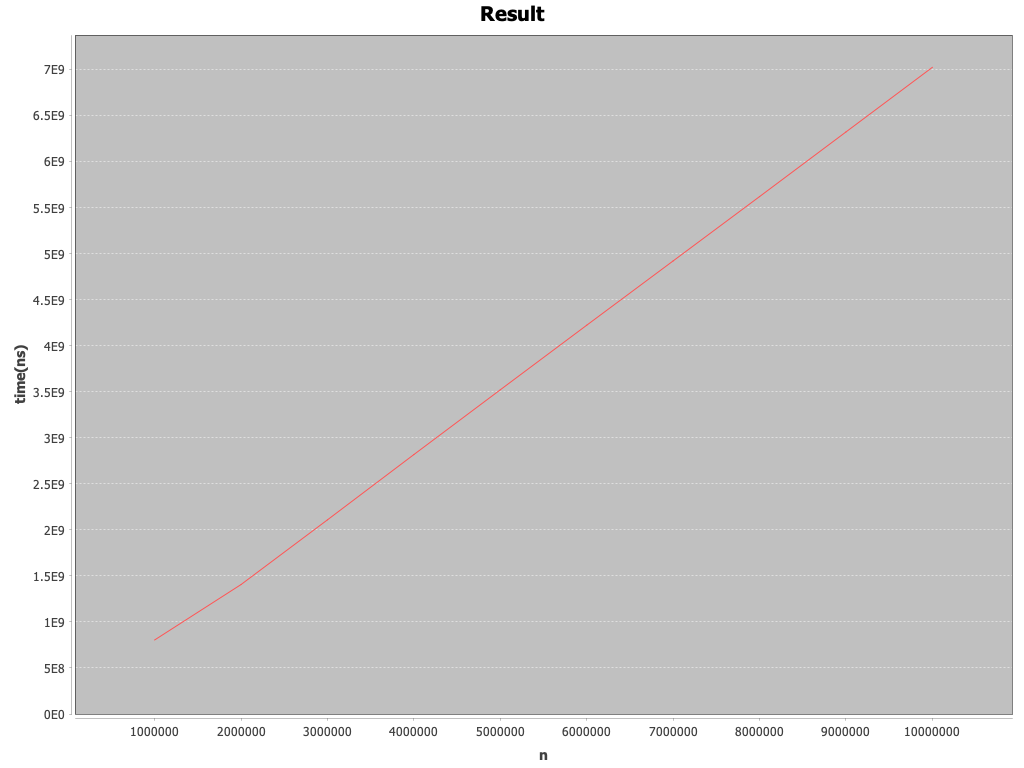
\includegraphics[width=0.8\textwidth]{Problem1.png}.\\
    The axes are linear in scale so a linear relationship looks like a line.\\
    \item Describe how the running times support your analysis of the asymptotic running times.\\
    When the input size doubles ($n = 5000000$ to $ 1000000$), the running time essentially doubles ($f(500000)= 3520291458 ns$ to $f(10000000) = 7021779542 ns$), which support the asymptotic analysis of $\Theta(n)$.\\
\end{enumerate}
\item Include your source code with your submission.\\
Here is the code in Java: The highlighted code is the tested code.
\begin{minted}[frame=lines,framesep=2mm,baselinestretch=1.2,fontsize=\footnotesize,linenos]{java}
import java.util.Arrays;

import org.jfree.chart.ChartFactory;
import org.jfree.chart.ChartFrame;
import org.jfree.chart.JFreeChart;
import org.jfree.chart.plot.PlotOrientation;
import org.jfree.data.category.DefaultCategoryDataset;

public class Hw2_p1 {
    public static void main(String[] args) {
        int n1 = 1000000;
        int n2 = 2000000;
        int n3 = 3000000;
        int n4 = 4000000;
        int n5 = 5000000;
        int n6 = 6000000;
        int n7 = 7000000;
        int n8 = 8000000;
        int n9 = 9000000;
        int n10 = 10000000;
        long[] result = new long[10];
        result[0] = time_calculate(n1);
        result[1] = time_calculate(n2);
        result[2] = time_calculate(n3);
        result[3] = time_calculate(n4);
        result[4] = time_calculate(n5);
        result[5] = time_calculate(n6);
        result[6] = time_calculate(n7);
        result[7] = time_calculate(n8);
        result[8] = time_calculate(n9);
        result[9] = time_calculate(n10);

        System.out.println(Arrays.toString(result));

        DefaultCategoryDataset dataset = new DefaultCategoryDataset();
        dataset.addValue(result[0],"time", "1000000");
        dataset.addValue(result[1],"time", "2000000");
        dataset.addValue(result[2],"time", "3000000");
        dataset.addValue(result[3],"time", "4000000");
        dataset.addValue(result[4],"time", "5000000");
        dataset.addValue(result[5],"time", "6000000");
        dataset.addValue(result[6],"time", "7000000");
        dataset.addValue(result[7],"time", "8000000");
        dataset.addValue(result[8],"time", "9000000");
        dataset.addValue(result[9],"time", "10000000");

        JFreeChart chart = ChartFactory.createLineChart(
                "Result",
                "n",
                "time(ns)",
                dataset,
                PlotOrientation.VERTICAL,
                false,true, false
        );

        ChartFrame chartFrame = new ChartFrame("Test", chart);
        chartFrame.pack();;
        chartFrame.setVisible(true);

    }

    public static void hello(int n){
        for (int i = 0; i < n; i++){
            // println is constant, c, and called n times
            System.out.println("Hello world");
        }
    }
    // A function representing time, f(n) = c * n;
    // f(n) is $\theta(n)$

    public static long time_calculate(int n){
        long startTime = System.nanoTime();
        hello(n);
        long endTime = System.nanoTime();
        long time = endTime - startTime;
        return time;
    }
}
\end{minted}

\end{enumerate}
    \end{sol}
    \item (50 pts) Write a program that takes a value ``$n$" as input; produces ``$n$" random numbers with a uniform distribution between $1$ and $n$ and places them in a singly linked list in sorted order.  Place them in the list in order, do not sort the list after placing them there.  You must have the list source code in your program. You may not use a ``built-in" list class or library. You may download the list source code from the internet.
    \begin{sol}
    ~\
    \begin{enumerate}
        \item From an analysis of your code, give a function representing the running time of your code. Give a tight asymptotic bound for that function. 
\begin{minted}[frame=lines,framesep=2mm,baselinestretch=1.2,fontsize=\footnotesize,linenos]{java}
    public static int[] Random_array(int n){
        Random rand = new Random(); // c1, 1 time
        int[] rand_number = new int[n]; // c2, 1 time
        for (int i = 0; i < n; i++){ // c3, (n + 1) times
            rand_number[i] = rand.nextInt(n+1);
            // rand.nextInt is constant, c4, and called n times
        }
        return rand_number; // c4, 1 times
        // A function representing time, f(n)= c1 * 1 + c2 * 1 
        // + c3*(n+1) + c4*n;
        // f(n) = $\Theta(n)$
    }

    public static int[] sort(int[] array){
        for (int j = 1; j < array.length; j++){ // c1, n time
            int key = array[j]; // c2, n-1 times
            int i = j-1; // c3, n-1 times
            while(i >= 0 && array[i] > key){ // c4, \sum_{j=1}^{n}tj
                array[i+1] = array[i]; // c5, \sum_{j=1}^{n}(tj-1)
                i = i - 1; // c6, \sum_{j=1}^{n}(tj-1)
            }
            array[i+1] = key; // c7, n-1
        }
        return array; // c8, 1 time
        // A function representing time, f(n)= c1 * n + c2 * (n-1) 
        // + c3*(n-1) + c4*\sum_{j=1}^{n}tj  
        // + c5*\sum_{j=1}^{n}(tj-1) 
        // + c6*\sum_{j=1}^{n}(tj-1) + c7 * (n-1);
        // f(n) = $\Theta(n^2)$
        // tj is constant
    }

    public static ListNode linkedlist(int[] array){
        ListNode root = new ListNode(array[0]); // c1, 1 time;
        ListNode ptr; // c2, 1 time
        ptr = root; // c3, 1 time
        int len = array.length; // c4, 1 time
        for (int i = 1; i < len; i++){ // c5, n times
            ptr.next = new ListNode(array[i]); // c6, n-1 times
            ptr = ptr.next; // c7, n-1 times
        } 
        return root;// c8, n-1 
        // A function representing time, f(n) = c1*1+ c2*1+ c3*1
        // +c4*1 + c5*n + c6*(n-1)+ c7*(n-1)+c8*(n-1)
        // f(n) = $\Theta(n)$
    }
    // f(n)= $\Theta(n) + \Theta(n^2)+\Theta(n)$ =\Theta(n^2)

\end{minted}
There are three function here, the first one is $Random\_array()$ function and then $sort()$ function and the 
third is $linkedlist()$ function: 
\begin{align*}
    f_1(n) &= c_1 \times 1 + c_2 \times 1  + c_3\times(n+1) + c_4\times n \\
    & = c_1+c_2 + c_3 + n(c_3+c_4) \\
    & =\Theta(n);\\
    f_2(n) & = c_1n + c_2(n-1) 
         + c_3(n-1) + c_4\sum_{j=1}^{n}t_j  
        + c_5\sum_{j=1}^{n}(t_j-1) 
         + c_6\sum_{j=1}^{n}(t_j-1) + c_7(n-1)\\
   & = c_1n + c_2(n-1)+c_3(n-1) + c_4(\frac{n(n+1)}{2}) + c_5(\frac{n(n-1)}{2}) + c_6(\frac{n(n-1)}{2}) + c_7(n-1)\\
   & = (\frac{c_4}{2}+\frac{c_5}{2}+\frac{c_6}{2})n^2+(c_1+c_2+c_3+\frac{c_4}{2}-\frac{c_5}{2}-\frac{c_6}{2}+c_7)n -
        (c_2+c_3+c_7)\\
   & = \Theta(n^2)\\
   f_3(n) & = c_1\times 1+ c_2\times 1 + c_3\times 1
        +c_4\times 1 + c_5\times n + c_6\times(n-1)+ c_7\times(n-1)+c_8\times (n-1)\\
        & = (c_5 + c_6 + c_7 + c_8)n + (c_1+c_2+c_3+c_4+c_5-c_6-c_7-c_8)\\
        & = \Theta(n)\\
   f(n) & = f_1+f_2+f_3 = \Theta(n^2)
\end{align*}
A function representing time: $f(n)$ is $\Theta(n^2)$ \\
\item Run your code for various values of $n$ and time it
\begin{enumerate}
    \item Create a graph of the running times vs various values of $n$. Use a linear scale on the axes.\\
    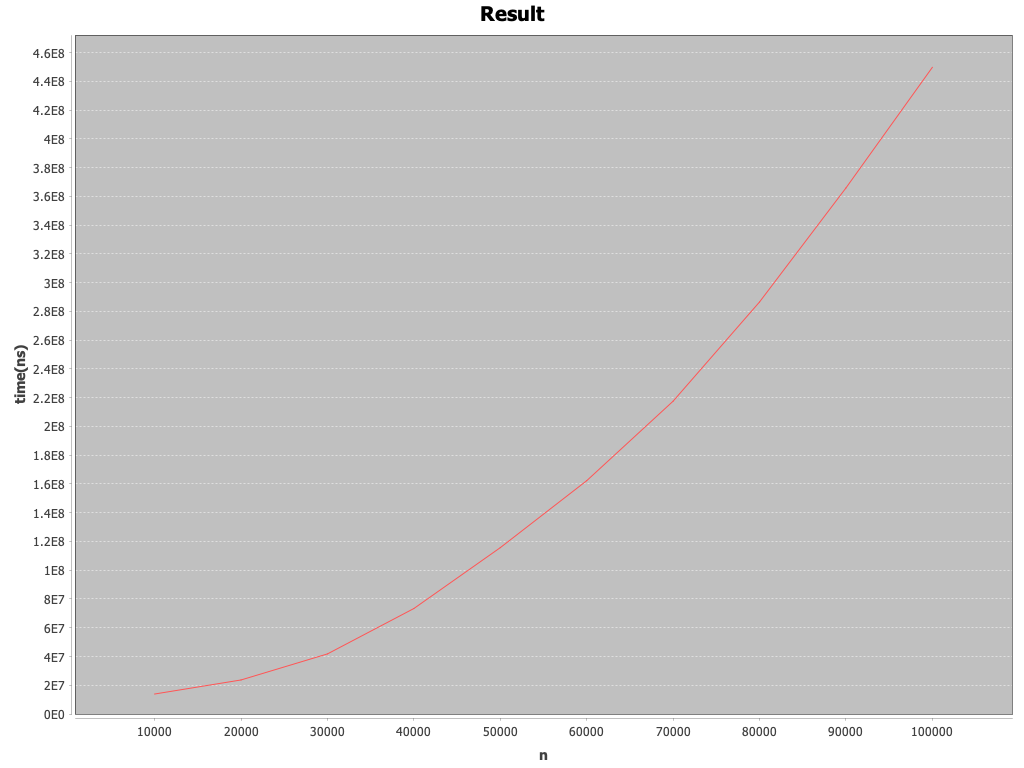
\includegraphics[width=0.8\textwidth]{Problem2.png}\\
    The axes are quadratic in scale so a quadratic relationship looks like a parabola.\\

    \item Create a chart showing the running times for various values of ``$n$"
    \begin{center}
    \begin{tabular}{c|c}
    \hline
    n & times(ns)  \\
    \hline 
    10000 & 13897125\\
    \hline
    20000 & 23677209 \\
    \hline
    30000 & 41795417 \\
    \hline
    40000 & 73369875 \\
    \hline 
    50000 & 115704709 \\
    \hline
    60000 & 162272584 \\
    \hline 
    70000 & 217587250 \\
    \hline 
    80000 & 286579209 \\
    \hline 
    90000 & 365880666 \\
    \hline
    100000 & 449781291 \\
    \hline
    \end{tabular}
    \end{center}\\
\item Describe how the running times support your analysis of the asymptotic running times.\\
    When the input size doubles ($n = 5000$ to $ 10000$), the running time essentially $2^2=4$ times ($f(5000)= 115704709 ns$ to $f(10000) = 449781291 ns$), which support the asymptotic analysis of $\Theta(n^2)$\\

\end{enumerate}

\item Include your source code with your submission.\\
Here is the code in Java: The highlighted code is the tested code.
\begin{minted}[frame=lines,framesep=2mm,baselinestretch=1.2,fontsize=\footnotesize,linenos]{java}
import org.jfree.chart.ChartFactory;
import org.jfree.chart.ChartFrame;
import org.jfree.chart.JFreeChart;
import org.jfree.chart.plot.PlotOrientation;
import org.jfree.data.category.DefaultCategoryDataset;

import java.util.Arrays;
import java.util.Random;

public class Hw2_p2 {
    public static class ListNode{
        public int value;
        public ListNode next;
        public ListNode(int value){
            this.value = value;
            next = null;
        }
    }

    public static void main(String[] args){
        int n1 = 10000;
        int n2 = 20000;
        int n3 = 30000;
        int n4 = 40000;
        int n5 = 50000;
        int n6 = 60000;
        int n7 = 70000;
        int n8 = 80000;
        int n9 = 90000;
        int n10 = 100000;
        long[] result = new long[10];
        result[0] = time_calculate(n1);
        result[1] = time_calculate(n2);
        result[2] = time_calculate(n3);
        result[3] = time_calculate(n4);
        result[4] = time_calculate(n5);
        result[5] = time_calculate(n6);
        result[6] = time_calculate(n7);
        result[7] = time_calculate(n8);
        result[8] = time_calculate(n9);
        result[9] = time_calculate(n10);
        System.out.println(Arrays.toString(result));

        DefaultCategoryDataset dataset = new DefaultCategoryDataset();
        dataset.addValue(result[0],"time", "10000");
        dataset.addValue(result[1],"time", "20000");
        dataset.addValue(result[2],"time", "30000");
        dataset.addValue(result[3],"time", "40000");
        dataset.addValue(result[4],"time", "50000");
        dataset.addValue(result[5],"time", "60000");
        dataset.addValue(result[6],"time", "70000");
        dataset.addValue(result[7],"time", "80000");
        dataset.addValue(result[8],"time", "90000");
        dataset.addValue(result[9],"time", "100000");

        JFreeChart chart = ChartFactory.createLineChart(
                "Result",
                "n",
                "time(ns)",
                dataset,
                PlotOrientation.VERTICAL,
                false,true, false
        );

        ChartFrame chartFrame = new ChartFrame("Test", chart);
        chartFrame.pack();;
        chartFrame.setVisible(true);

    }

    public static int[] Random_array(int n){
        Random rand = new Random();
        int[] rand_number = new int[n];
        for (int i = 0; i < n; i++){
            rand_number[i] = rand.nextInt(n+1);
        }
        return rand_number;
    }

    public static int[] sort(int[] array){
        for (int j = 1; j < array.length; j++){
            int key = array[j];
            int i = j-1;
            while(i >= 0 && array[i] > key){
                array[i+1] = array[i];
                i = i - 1;
            }
            array[i+1] = key;
        }
        return array;
    }

    public static ListNode linkedlist(int[] array){
        ListNode root = new ListNode(array[0]);
        ListNode ptr;
        ptr = root;
        int len = array.length;
        for (int i = 1; i < len; i++){
            ptr.next = new ListNode(array[i]);
            ptr = ptr.next;
        }
        return root;
    }

    public static void display(ListNode root){
        while(root != null){
            System.out.print(root.value + " ");
            root = root.next;
        }
    }

    public static long time_calculate(int n){
        long startTime = System.nanoTime();
        int[] array = Random_array(n);
        int[] sortarray = sort(array);
        ListNode listNode = linkedlist(sortarray);
        long endTime = System.nanoTime();
        long time = endTime - startTime;
        return time;
    }
}

\end{minted}
\end{enumerate}
    
\end{sol}
\end{enumerate}
Turn in your assignment as a single pdf file with the answers and source code for all problems.
\end{document}
